\section{System Architecture Design}

In the following we will specify our main components that execute our main functionalities. All components are separated into the following Layers according to ISO/OSI Model.

\begin{figure}
    \centering
    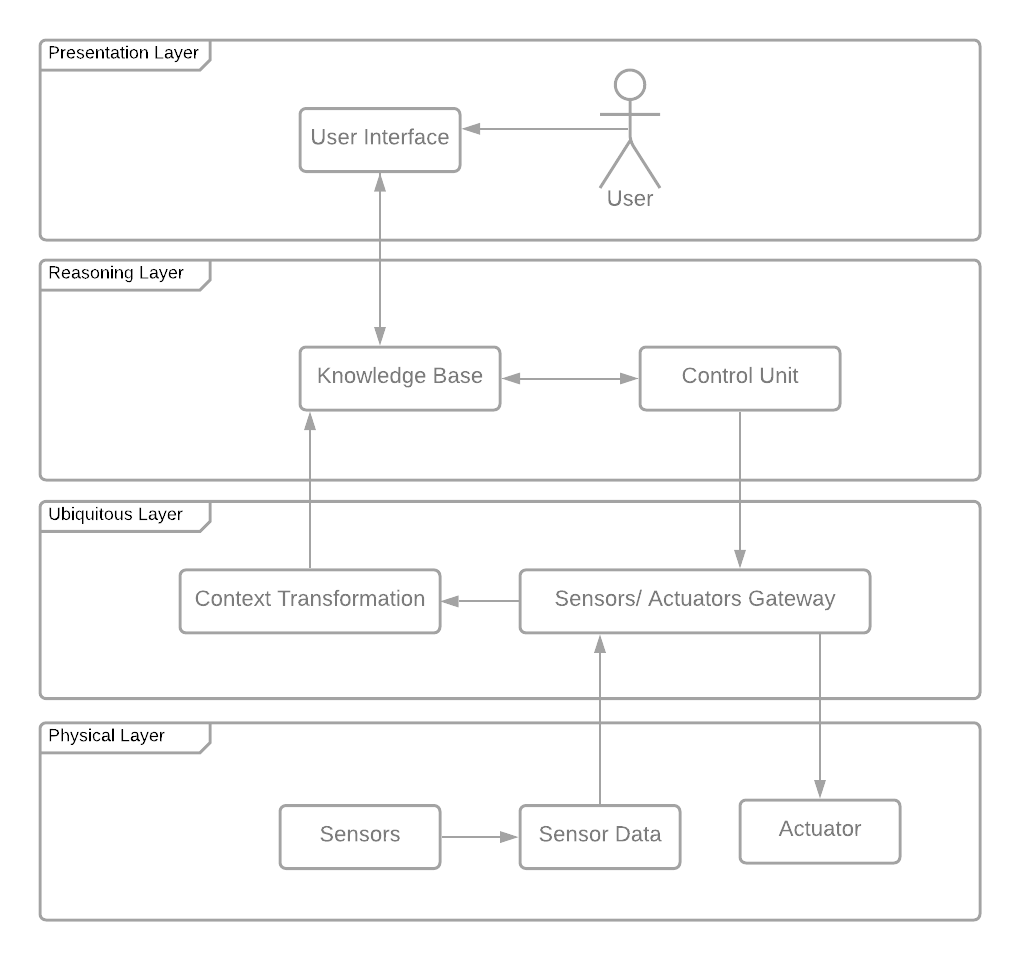
\includegraphics[width=\linewidth]{img/system-design.png}
    \caption{The system design illustrated as a diagram}
    \label{fig:system-design}
\end{figure}

\subsection{Presentation Layer}
The Presentation Layer consists of the User Interface and the User itself. The (human) User interacts with our system via the User Interface which is a GUI. The user can monitor the system as described in functional requirement FA-5.

\subsection{Reasoning Layer}
The reasoning layer consists of the knowledge base and the control unit. The knowledge base stores all the sensor data that is generated and stores information about the individual room with the state of all the actuators. It receives all its data from the Context Transformation component in the Ubiquitous Layer. The Control Unit interacts closely with the Knowledge Base, as it receives a notification as soon as new sensor data is stored in the Knowledge Base. Based on all the data, the Control Unit decides based on AI-planning what actions it should take next. As soon as it has reached a conclusion and formulated a plan, it communicates this plan with the Sensors/Actuators gateway in the Ubiquitous Layer.

\subsection{Ubiquitous Layer}
The main component of the ubiquitous layer is the sensor/actuator gateway which communicates between the physical layer devices and the components of the reasoning layer. It will process commands from the control unit of the reasoning layer directly in order to relay commands to the actuators of the system. Sensor data however will be given to the Context Transformation component which has the job to take this raw data and transform it to a more precise and informative format which will then be communicated with the knowledge base of the reasoning layer.

\subsection{Physcial Layer}
There are two main components of the physical layer. Firstly the sensor which produces sensor data that will be sent to the gateway. Sensors will be used to satisfy functional requirements such as FA-8 and others. Secondly actuators will get instructions from the gateway and execute upon these as is described in the functional requirements.
